\chapter{Biological Background}\label{chapter:biology}

Sounds\dots{} For sure, they are one of the most important sources of information in our everyday life. By listening to them, one can describe what is happening around, understand how to react to occurring situations, or even tell if a danger is approaching, and it is time to take action. It is hard to imagine human sensation without hearing, but as easy as this may sound (no pun intended), the~biology behind it is quite complicated. This chapter will introduce the reader to how sound as a~mechanical phenomenon is converted to sound as perception and provide a~basic overview of the structures in the human ear, along with the mechanical and neurobiological processes happening inside of them.

\section{Outer and Middle Ear}

At the beginning, sound approaches the ear by vibrations in the air (or any other elastic medium) and enters the outer ear, which consists of the visible part (called the auricle, or the pinna) and the ear canal. The auricle is a thin plate of elastic cartilage, covered with integument, and connected to the surrounding parts by ligaments and muscles; and to the beginning of the ear canal by fibrous tissue [Wikipedia citation – Outer ear]. The ear canal is a tube leading from the~bottom of the~auricle to the middle ear, separated from it by the eardrum (or tympanic membrane). The main purpose of the ear canal is to focus the sound energy gathered by the auricle on the~eardrum. It also amplifies frequencies between 3\,kHz and 12\,kHz.\\

Being gathered on the eardrum, the mechanical vibrations propagate through the middle ear. Three bones (called the ossicles) are located inside of it. The malleus (also called the hammer) is connected to the eardrum and transfers the vibrations from it to the incus (the anvil). These vibrations are quite chaotic, but the malleus is connected to the eardrum in a linear manner, also helping the ear to respond more linearly and smoothly. The incus, in turn, connects to the stapes (the stirrup). The footplate of the stapes introduces pressure waves in the inner ear, which starts with the oval window of the cochlea. The structures of the middle ear can be seen on Figure~\ref{img:anatomy_human_ear}\\

\begin{figure}[h]
	\centering
	\begin{subfigure}{0.5\textwidth}
		\centering
		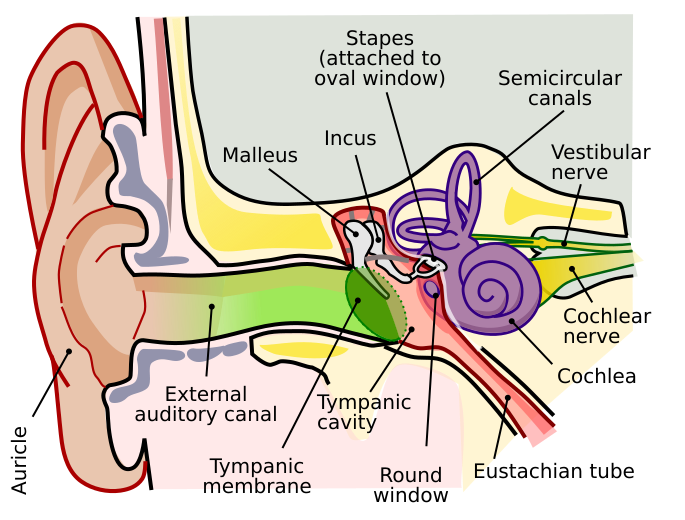
\includegraphics[width=\linewidth]{include/anatomy_of_the_human_ear}
		\caption{}
		\label{img:anatomy_human_ear}
	\end{subfigure}%
	\begin{subfigure}{0.5\textwidth}
		\centering
		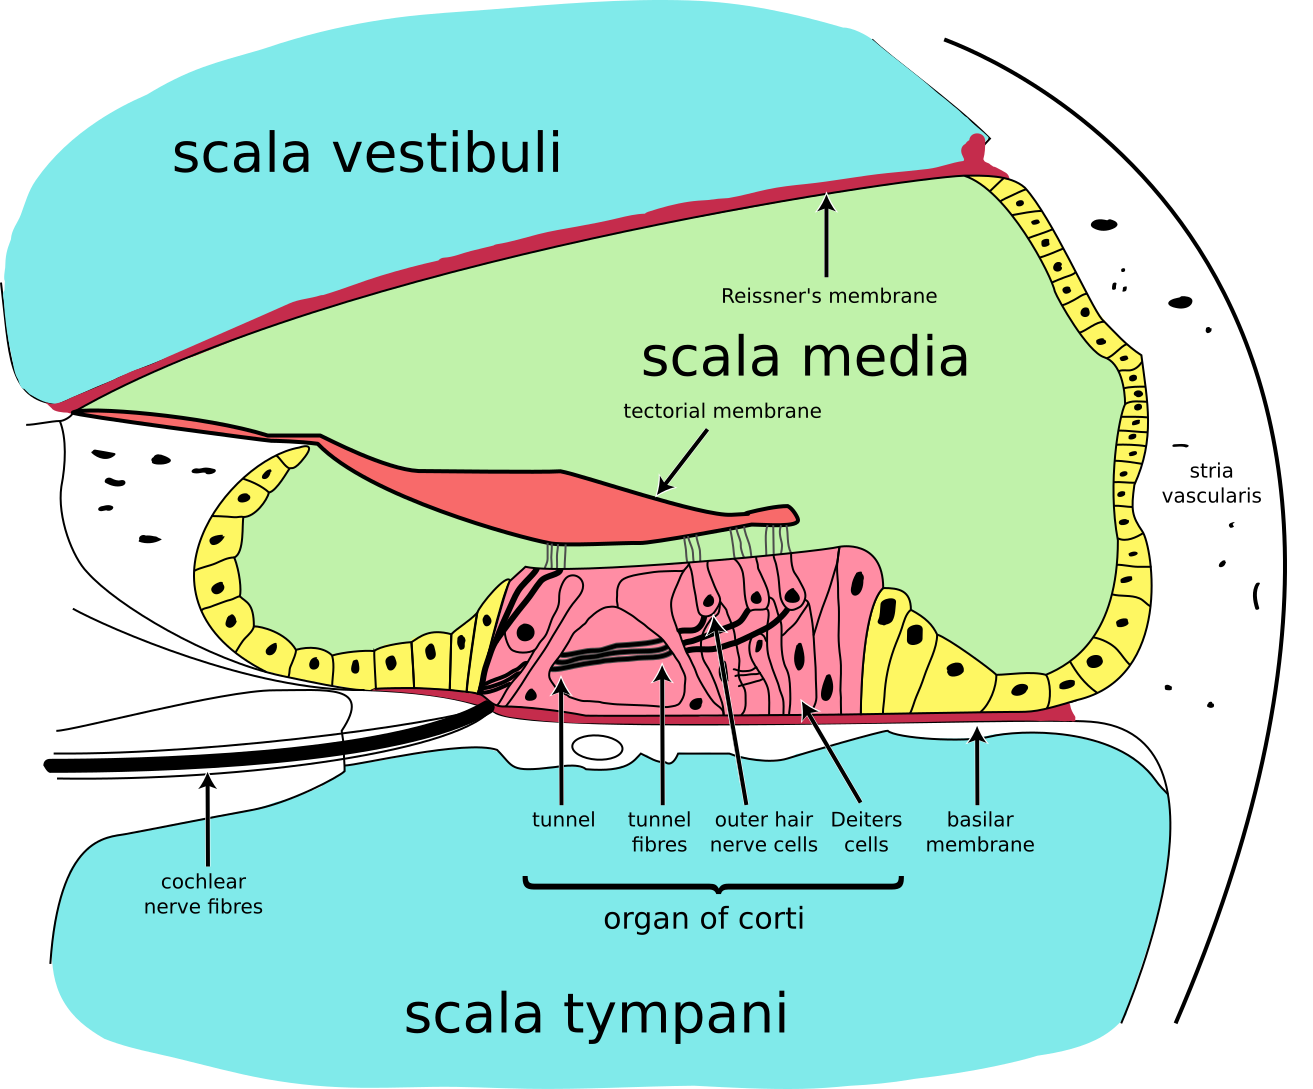
\includegraphics[width=\linewidth]{include/cochlea_cross_section}
		\caption{}
		\label{img:cochlea_cross_section}
	\end{subfigure}
	\caption[Anatomy of the human ear]{\textbf{(a)} Anatomy of the human ear. The ossicles of the middle ear are shown in white. The inner ear is shown in purple. \textbf{(b)} Cross-section of the cochlea showing the organ of Corti and three chambers filled with cochlear fluids. Both pictures were taken from \url{{https://commons.wikimedia.org/}}}
\end{figure}

It may sound redundant to have additional structures in the ear which propagate the vibrations even further, when they could travel just one centimeter more in a way like before, in the ear canal, but in reality, the pressure of these mechanical vibrations is too small to cause the waves of the same velocity in the cochlear fluids. The ossicles help to amplify the pressure of these vibrations. They are positioned to form a lever, and, because the oval window is about 14~times smaller than the eardrum, the pressure gain becomes quite significant in the end -- at~least 18.1~times [Wikipedia citation – Middle ear].\\

To regulate the middle ear and protect it from damage due to very loud sounds, two muscles are located inside of it: the stapedius muscle and the tensor tympani muscle. These muscles are controlled by unconscious reflexes and hold the ossicles when the vibrations become too intense. To provide ventilation and drainage of the middle ear and to equalize pressures in this isolated environment, the middle ear is connected to the back of the throat by the eustachian tube \cite{Schnupp2011}.

\section{Inner Ear}

The inner ear starts with the above-mentioned oval window, which is connected to the stapes of the middle ear. The oval window is a part of the cochlea –- a structure of the inner ear dedicated to hearing. Along with the cochlea, the inner ear also contains the vestibular system, which is responsible for the sense of balance and spatial orientation and uses the same kinds of fluids and cells as the cochlea does. The vestibular system will not be covered in this thesis, but the fluids and cells will be described in more detail later in the section.\\

The cochlea itself is a spiral-shaped cavity made of bony tissue, which makes about 2.75~turns around its axis and is about 3\,cm long [Wikipedia citation - Cochlea]. The core component of it is the basilar membrane, which runs along almost its entire length and separates two of the three chambers of the cochlea filled with different fluids: the tympanic duct filled with perilymph (scala tympani), and the cochlear duct filled with endolymph (scala media). The third chamber, the vestibular duct (scala vestibuli), is separated from the cochlear duct by the Reissner’s membrane and is filled with perilymph (Figure~\ref{img:cochlea_cross_section}). When the footplate of the stapes of the middle ear introduces movements to the cochlear fluids, the basilar membrane is affected too, and the endolymph in the cochlear duct moves along.\\

The most interesting property of the basilar membrane is that its stiffness and width is different throughout its length – the membrane is narrow and stiff at the basal end of the cochlea, and wide and floppy at the apical end. And here sound waves have two possible routes to take while propagating through the basilar membrane: a shorter path, which includes going through the stiffer parts of it, or a longer path, which means travelling along the membrane until it becomes easier to pass through, but pushing more fluid on the way. In fact, high-frequency waves tend to choose the shorter path, and low-frequency waves – the longer one.\\

Thus, the basilar membrane moves in different places depending on the frequencies of the vibrations. The organ of Corti, which sits on top of it and runs along its entire length, contains displacement cells able to respond to movements of the fluid nearby and send electrical impulses when this happens. Such cells are packed with a bunch of stereocilia (hair) that stick out of its top, and thus are called hair cells. These cells can be of two types: inner hair cells that are located closer to the center of the cochlea, and outer hair cells that sit closer to its outer side. Inner hair cells are less numerous than outer hair cells and form a single row along the organ of Corti, while outer hair cells usually form three rows \cite{Schnupp2011}.\\

Now, it is important to mention that the endolymph in the cochlear duct contains high amounts of positively charged ions (primarily potassium and calcium). When it moves in response to the sound pressure, the stereocilia of the inner hair cells are deflected, and tiny ion channels open in them. This allows the charged ions from the endolymph to enter the stereocilia. The cell becomes depolarized, and a receptor potential is produced. This results in releasing the neurotransmitters at the basal end of the cell and then triggering action potentials in the nerve nearby. In this way, inner hair cells detect movements around them and convert mechanical sound waves to electrical nerve signals.\\

Outer hair cells, in turn, serve as amplifiers of the quiet sounds. Their receptor potentials are converted to cell body movements, thus increasing the sound pressure \cite{Hudspeth2008}.

\section{Auditory Scene Analysis}\label{section:biology_asa}

